\documentclass[11pt]{article}
\usepackage[a4paper,margin=2.6cm]{geometry}
\usepackage{amsmath,amssymb,bm}
\usepackage{tikz}
\usetikzlibrary{positioning,arrows.meta}
\usepackage{booktabs}
\usepackage{xcolor}
\usepackage[colorlinks=true,linkcolor=blue!50!black,citecolor=blue!50!black]{hyperref}
\usepackage{tcolorbox}
\tcbset{colback=gray!5,colframe=gray!40,boxrule=0.4pt,left=6pt,right=6pt,top=4pt,bottom=4pt}

\newcommand{\h}{\bm{h}}
\newcommand{\R}{\mathbb{R}}
\newcommand{\E}{\mathbb{E}}
\newcommand{\dBC}{d_{\mathrm{BC}}}

\title{\textbf{Neural geometry of an RL agent's beliefs and behavior:\\ methods}}
\author{}
\date{}

\begin{document}
\maketitle
\vspace{-3em}

\begin{abstract}
\noindent
This document specifies, step by step, the analysis pipeline we use to expose
the \emph{belief}, \emph{decision} and \emph{behavior} structure inside a
recurrent RL agent. The pipeline constructs three objects --- a \textbf{belief
space} (distributions over the latent task variable), a \textbf{behavior space}
(distributions over future outcomes), and an \textbf{activation manifold} (the
geometry of the hidden states that carry both) --- and then intervenes on them
in both directions: editing beliefs to change behavior, and forcing behavior to
change beliefs. Every technique operates on plain arrays
$(\text{hidden states},\ \text{labels},\ \text{progress},\ \text{distributions})$
and is therefore portable to any navigation-and-decision environment; the only
environment-specific component is the data-collection layer.
\end{abstract}

\section{Setting and notation}

An agent with a recurrent policy interacts with a POMDP. At time $t$ it
receives an observation $o_t$, updates its hidden state
\begin{equation}
  \h_t \;=\; F(\h_{t-1},\, o_t) \in \R^{d},
\end{equation}
(here $F$ is a GRU, $d{=}256$) and samples an action $a_t \sim \pi(\cdot \mid
\h_t)$. The environment contains a \emph{latent task variable} $c$ (in
MemoryEnv: the cue identity, $c \in \mathcal{C}$, which factorizes into
direction and color) that is observable only during a brief window, and is
\emph{consumed} by decisions much later. We also fix a scalar \textbf{progress
parameter} $x_t$ (in MemoryEnv: the agent's corridor column; in a noisier
environment any monotone task-progress proxy works, e.g.\ distance-to-goal or
a learned progress index).

\begin{tcolorbox}
\textbf{Portability requirements.} To run the pipeline on another environment
(e.g.\ the \texttt{bridge\_tunnel} navigation task) one must provide:
(i) rollouts with hidden states $\h_t$;
(ii) a label for the latent variable of interest $c$ (what the agent must
remember);
(iii) a progress parameter $x_t$;
(iv) a definition of terminal \emph{outcomes} $z$ (which decisions were taken).
Nothing else in the pipeline changes.
\end{tcolorbox}

\begin{figure}[h]
\centering
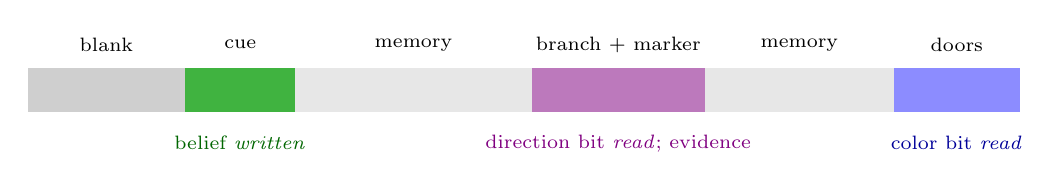
\begin{tikzpicture}[x=1cm,y=1cm]
\foreach \a/\b/\nm/\col in {0/2/blank/gray!50, 2/3.4/cue/green!60!black,
  3.4/6.4/memory/gray!25, 6.4/8.6/{branch + marker}/violet!70,
  8.6/11/memory/gray!25, 11/12.6/doors/blue!60}{
  \fill[\col,opacity=.75] (\a,0) rectangle (\b,.55);
  \node[font=\scriptsize] at ({(\a+\b)/2},.85) {\nm};
}
\node[font=\scriptsize,green!40!black] at (2.7,-.4) {belief \emph{written}};
\node[font=\scriptsize,violet] at (7.5,-.4) {direction bit \emph{read}; evidence};
\node[font=\scriptsize,blue!60!black] at (11.8,-.4) {color bit \emph{read}};
\end{tikzpicture}
\caption{One episode as a memory pipeline: a two-bit belief is written once,
carried, and its bits are spent at two different decision points. The
mid-corridor marker door provides branch-identity \emph{evidence} that the
agent experiences en route.}
\end{figure}

\section{Data collection}

\paragraph{Traces.} We roll the \emph{stochastic} policy (actions sampled from
the softmax) for $n$ episodes per training cue and store, per live step, the
tuple $(\h_t, x_t, c, t, \text{cue-seen}_t)$, where
$\text{cue-seen}_t$ flags whether the cue has entered the agent's egocentric
view at any $t' \le t$. Sampling (rather than greedy) matters: it broadens the
state distribution around each trajectory, which manifold fitting and probing
need; greedy rollouts collapse onto a handful of paths.

\paragraph{Alignment convention.} $\h_t$ is the hidden state \emph{after}
processing $o_t$; the pair $(\h_t, s_{t+1})$ --- belief after seeing $o_t$,
environment state after acting --- is the correct point to resume simulation
from (used by the Monte-Carlo behavior estimates below).

\section{Belief space}

\paragraph{Probe.} A multinomial logistic probe estimates the agent's posterior
over the latent variable from the hidden state:
\begin{equation}
  P(c \mid \h) = \mathrm{softmax}\!\big(W\h + \bm b\big)_c ,
\end{equation}
trained with cross-entropy + $\ell_2$ on trained-cue states. Crucially the
class set is $\mathcal{C} \cup \{\varnothing\}$: a \textbf{blank class} of
pre-cue states ($\text{cue-seen}=\text{false}$). Without it the probe must
extrapolate on pre-cue states that lie off its training manifold, and logistic
extrapolation is confident by construction --- producing the artifact that
``the belief is already decided before the cue''. With the blank class,
$P(\varnothing\mid\h)\!\approx\!1$ before the cue and control transfers to the
cue classes exactly at cue onset (\S\ref{sec:precue}).

\paragraph{The space.} Each state now maps to a point on the probability
simplex $\Delta^{|\mathcal C|}$. We call the image of the data under
$\h \mapsto P(\cdot\mid\h)$ the \emph{belief space}.

\section{Behavior space}

The behavior of a state is not its next action but the \emph{distribution over
futures} it induces. For a stratified subset of states (a few per progress
column per cue) we resume the environment from $(\h_t, s_{t+1})$ and roll the
stochastic policy $K$ times ($K{=}24$), recording the terminal outcome
$z \in \{\text{up},\text{down}\}\times\{\text{green},\text{blue}\}$:
\begin{equation}
  \widehat{P}(z \mid \h_t)
  \;=\; \tfrac1K \textstyle\sum_{k=1}^K \mathbf 1\!\left[z^{(k)} = z\right].
\end{equation}
This \textbf{Monte-Carlo outcome posterior} lives on $\Delta^{4}$ and defines
the \emph{behavior space}. Early states have high-entropy behavior only through
policy stochasticity; after each decision is spent, outcome mass collapses ---
the geometry of the behavior space literally displays decision-making.

\section{inPCA: embedding spaces of distributions}
\label{sec:inpca}

Belief and behavior points are probability vectors, so Euclidean PCA is the
wrong geometry. We embed them with \emph{intensive PCA}
(inPCA; Quinn et al., PNAS 2019), the technique used in Goodfire's
``Shape of Beliefs''. Given points $\{p^{(i)}\}$, form the pairwise
Bhattacharyya divergence
\begin{equation}
  D_{ij} \;=\; -\log \textstyle\sum_k \sqrt{p^{(i)}_k\, p^{(j)}_k},
\end{equation}
double-center it, $W = -\tfrac12 J D J$ with $J = I - \tfrac1n \bm 1\bm 1^\top$,
and eigendecompose $W = V \Lambda V^\top$. Coordinates are
$V\sqrt{|\Lambda|}$, keeping eigenvalues \emph{signed}: inPCA is an isometric
embedding into Minkowski space (negative-$\lambda$ directions are
``time-like''); in practice the leading components are positive and the plot
reads like PCA but with distances that are faithful to probability space.
Where only a metric (not a visualization) is needed we use the closed-form
\textbf{Hellinger map} $p \mapsto \sqrt{p}$, under which the simplex embeds
almost-Euclideanly ($d_H^2(p,q) = \sum_k (\sqrt{p_k}-\sqrt{q_k})^2$).

\begin{tcolorbox}
\textbf{Why not UMAP/t-SNE?} Both are non-parametric: they cannot project
\emph{new} states (e.g.\ steered, off-distribution ones) faithfully, they
distort distances by design, and their layout is fit-dependent --- all fatal for
before/after intervention comparisons. Every projection we use (probes, PCA,
inPCA, Hellinger) is parametric and out-of-sample-safe.
\end{tcolorbox}

\section{The activation manifold: a tree of fibers}
\label{sec:tree}

For each cue $c$ and progress bin $x$ compute the centroid
$\mu_c(x) = \E[\h \mid c, x, \text{cue seen}]$, and for pre-cue states the
cue-independent centroid $\mu_\varnothing(x)$. Connecting centroids along $x$
yields polyline \emph{fibers}, one per cue, plus a shared pre-cue
\emph{trunk}: the activation manifold of this task family is a
\textbf{tree} (Fig.~\ref{fig:tree}). Fiber arc-length
$s_c(x) = \sum_{x' \le x} \lVert \mu_c(x'{+}1) - \mu_c(x') \rVert$ gives
geodesic distances \emph{on} the manifold:
\begin{equation}
  d_{\mathrm{tree}}\big((c,x),(c',x')\big) =
  \begin{cases}
    |s_c(x) - s_c(x')| & c = c'\\[2pt]
    s_c(x) + s_{c'}(x') & c \neq c' \quad (\text{path through the split}),
  \end{cases}
\end{equation}
with arcs measured from the split point (cue-room exit). Splines can replace
polylines when bins are dense; for noisier environments the same construction
applies with soft binning of $x$.

\begin{figure}[h]
\centering
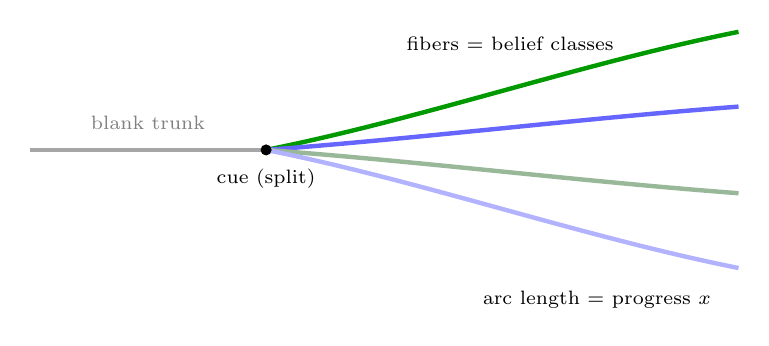
\begin{tikzpicture}[x=1cm,y=1cm]
\draw[gray!70, line width=1.6pt] (0,0) .. controls (1.5,0) .. (3,0);
\draw[green!60!black, line width=1.6pt] (3,0) .. controls (5,.4) and (7,1.1) .. (9,1.5);
\draw[blue!60, line width=1.6pt]        (3,0) .. controls (5,.15) and (7,.4) .. (9,.55);
\draw[green!30!black!40, line width=1.6pt](3,0) .. controls (5,-.15) and (7,-.4) .. (9,-.55);
\draw[blue!30, line width=1.6pt]        (3,0) .. controls (5,-.4) and (7,-1.1) .. (9,-1.5);
\node[font=\scriptsize,gray] at (1.5,.35) {blank trunk};
\node[font=\scriptsize] at (6.1,1.35) {fibers = belief classes};
\node[font=\scriptsize] at (7.2,-1.9) {arc length = progress $x$};
\fill (3,0) circle (2pt); \node[font=\scriptsize,below] at (3,-.12) {cue (split)};
\end{tikzpicture}
\caption{The activation manifold as a trunk-and-fibers tree. ``Which fiber''
is the belief; ``where along the fiber'' is task progress. Geodesics between
fibers pass through the split.}
\label{fig:tree}
\end{figure}

\paragraph{Isometry test.} Following Goodfire's manifold-steering analysis we
correlate tree geodesics with distribution distances: for all node pairs, plot
$d_{\mathrm{tree}}$ against the Hellinger distance of the nodes' mean
\emph{belief} distributions and of their mean \emph{behavior} distributions.
The expected signature: belief distance is a step function of the tree (zero
within a fiber, saturated across fibers --- belief is \emph{which} fiber),
while behavior distance grows along fibers as decisions are consumed. This is
the geometric statement of the belief/behavior distinction.

\section{Linear field probes: does the memory code rotate?}
\label{sec:lfp}

A single probe assumes one global belief axis. A \emph{linear field probe}
(LFP; ``Shape of Beliefs'') is a family of probes indexed by progress: for
every bin $x$ fit a multinomial probe $W_x$ on the states \emph{in that bin
only}. Three diagnostics:
\begin{itemize}
  \item \textbf{Gram matrix} $K_{xx'} = \cos\big(\mathrm{vec}(W_x),
        \mathrm{vec}(W_{x'})\big)$: near-constant $\Rightarrow$ stationary
        code; banded/decaying $\Rightarrow$ the code \emph{rotates} with
        position;
  \item \textbf{transfer matrix} $T_{x\to x'}$: accuracy of the bin-$x$ probe
        evaluated at bin $x'$;
  \item \textbf{rotation angle} $\theta = \arccos K_{x_{\min} x_{\max}}$
        between the first and last probes.
\end{itemize}
A rotating code has a direct causal consequence: \emph{any single global
steering axis is the wrong axis somewhere along the corridor} --- the
explanation for interventions that decode perfectly yet fail causally.

\paragraph{Additivity.} The centroid grid also admits a factorization test:
fit $\mu_c(x) \approx m + a_c + b_x$ by least squares and report $R^2$. High
$R^2$ means memory content and progress are encoded in independent (additive)
subspaces; the residual quantifies their interaction.

\section{Interventions}
\label{sec:interventions}

\subsection{Belief $\to$ behavior: transient swaps, global vs field-aware}

A \textbf{global swap} implants cue $t$ into an episode of cue $s$ by clamping
the hidden state along the class-mean axis during a window $\mathcal W$
(cue-room exit until the branch decision; released afterwards):
\begin{equation}
  \h \leftarrow \h + \big(\rho - \h^\top \hat u\big)\,\hat u,
  \qquad
  \hat u = \frac{\mu_t - \mu_s}{\lVert \mu_t - \mu_s\rVert},\quad
  \rho = \mu_t^\top \hat u .
\end{equation}
The \textbf{field-aware swap} replaces the single axis with a
\emph{position-local} field: per-column axes
$\hat u(x) \propto \mu_t(x) - \mu_s(x)$ and targets
$\rho(x) = \mu_t(x)^\top \hat u(x)$, spline-smoothed across columns
(coordinate-wise), applied with the agent's current column $x_t$. If the code
rotates (\S\ref{sec:lfp}), only the field version tracks the manifold.

\paragraph{Path energy.} Interventions are scored not only by success
(``behaves as target'': target branch \emph{and} target door) but by
\emph{naturalness}: the mean Bhattacharyya distance of the probe posterior to
the target vertex during the window,
$E = \tfrac1{|\mathcal W|}\sum_{t\in\mathcal W}
\dBC\!\big(P(\cdot\mid\h_t),\, \delta_{t}\big)$ ---
Goodfire's manifold-energy criterion, discretized. Low energy means the edit
moved the state \emph{along} the belief manifold rather than through a void.

\subsection{Behavior $\to$ belief: forcing through evidence}

The converse intervention never touches $\h$: pure \emph{action replacement}
drives the agent through the direction-\emph{wrong} corridor, including opening
its marker door --- an observation that never co-occurs with the true cue in
training --- then releases control. Readouts: the probe posterior aligned at
the marker-opening event, the final door choice, and the \textbf{implied
evidence weight}
\begin{equation}
  \mathrm{LLR} = \log \frac{P(\text{destination cue}\mid \h_{\text{pre-door}})}
                           {P(\text{true cue}\mid \h_{\text{pre-door}})},
\end{equation}
measured at the last step before the final doors enter the agent's view (so
the readout reflects memory, not fresh door perception). A symmetric Bayesian
observer holding contradictory cue-vs-corridor evidence of equal reliability
sits at $\mathrm{LLR}=0$; $\mathrm{LLR}>0$ quantifies recency dominance.
Whether the belief \emph{collapses to another attractor} (entangled training
set) or \emph{revises one factor only} (factorized training set) is the
central comparative result.

\section{Attractor census}

Beliefs persist because they are attractors of the closed-loop dynamics. Fix a
neutral ``maintenance'' observation $o^\ast$ (mid-corridor, nothing salient in
view) and study the step map $\Phi(\h) = F(\h, o^\ast)$. Fixed points are found
by minimizing $\lVert \Phi(\h) - \h\rVert^2$ with Adam from a few hundred
data-adjacent initializations, merging duplicates; stability follows from the
spectral radius of the Jacobian $\partial\Phi/\partial\h$ at each point
($<\!1$: attractor). Each fixed point is identified with its nearest class
mean. The census (how many attractors, their stability margins, where the
saddles sit) explains asymmetries in steerability: a ``default'' cue is a
deeper attractor, and doses that fail to cross its basin boundary are erased
by the flow.

\paragraph{Flow-field panels.} For visualization we take a 2-D affine slice of
state space through the mean hidden state, spanned by orthonormalized probe
axes; each grid point of the slice is a genuine state $\h(u,v)$, colored by
the probe's decision regions and overlaid with the \emph{in-plane component} of
$\Phi(\h)-\h$ as arrows. (Caveat to keep in the figure caption: motion out of
the slice is invisible; the slice shows a section of a $d$-dimensional flow.)

\section{The pre-cue bias: diagnosis and fix}
\label{sec:precue}

\textbf{Symptom.} Probes report $P(\text{one cue}) \approx 1$ \emph{before}
the cue is visible. \textbf{Diagnosis.} Two stacked causes: (i) a probe
trained only on post-cue states is evaluated off its training manifold;
logistic regression partitions all of $\R^d$, so off-manifold points get
confident, arbitrary labels; (ii) genuinely, the pre-cue trunk lies closer to
one fiber --- the network's \emph{default basin} (an honest, measurable fact
about its dynamics, not a bug). \textbf{Fix (no retraining).} Add the blank
class (\S3) and report the distance-to-manifold
$d(\h) = \min_{\text{nodes}} \lVert \h - \mu \rVert$, normalized by the
on-manifold median, alongside every belief readout: pre-cue states then read
as ``blank'' and any steered state that leaves the manifold is flagged rather
than silently misread. A retraining fix (auxiliary calibrated-belief loss)
would inject representation supervision and break the emergent-concepts design
--- we deliberately do not use it.

\section{Summary of the pipeline}

\begin{center}
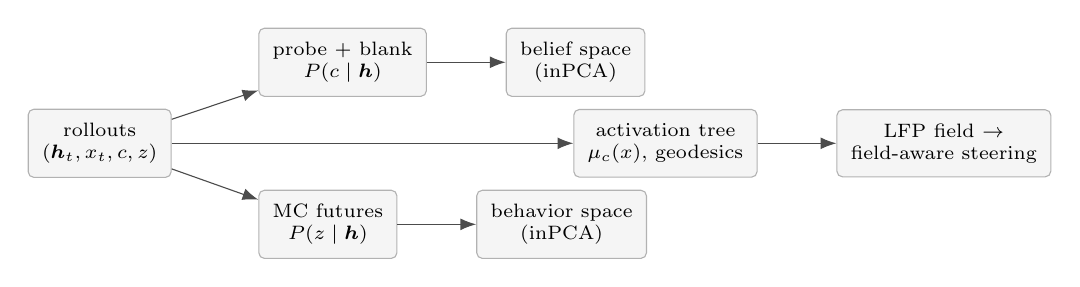
\begin{tikzpicture}[
  box/.style={draw=gray!60, fill=gray!8, rounded corners=2pt, inner sep=5pt,
              font=\scriptsize, align=center},
  arr/.style={-{Latex[length=2mm]}, gray!60!black}]
\node[box] (h)  {rollouts\\ $(\h_t, x_t, c, z)$};
\node[box, above right=0.15cm and 1.1cm of h] (probe) {probe + blank\\ $P(c\mid\h)$};
\node[box, below right=0.15cm and 1.1cm of h] (mc) {MC futures\\ $P(z\mid\h)$};
\node[box, right=1.0cm of probe] (bel) {belief space\\ (inPCA)};
\node[box, right=1.0cm of mc]  (beh) {behavior space\\ (inPCA)};
\node[box, right=5.1cm of h] (tree) {activation tree\\ $\mu_c(x)$, geodesics};
\node[box, right=1.0cm of tree] (steer) {LFP field $\to$\\ field-aware steering};
\draw[arr] (h) -- (probe); \draw[arr] (h) -- (mc);
\draw[arr] (probe) -- (bel); \draw[arr] (mc) -- (beh);
\draw[arr] (h) -- (tree); \draw[arr] (tree) -- (steer);
\end{tikzpicture}
\end{center}

\noindent The same seven analyses (belief space, behavior space, activation
tree, isometry, LFP/rotation, two-way steering with path energy, attractor
census) apply verbatim to any environment providing the four ingredients of
\S1 --- for \texttt{bridge\_tunnel}/cogniland the latent variable is the
committed skill and map category, progress is distance-to-target, and outcomes
are (skill used, target reached).

\end{document}
